\documentclass[a4paper,dvipsnames]{article}

\input ../header
\newcommand{\checkedbox}{\makebox[0pt][l]{$\square$}\raisebox{.15ex}{\hspace{0.1em}$\checkmark$}}
\newcommand{\checkbox}{\makebox[0pt][l]{$\square$}\raisebox{.15ex}{\hspace{0.1em}}\hspace{3mm}}

% Intervalle
\def\intervalleFF(#1,#2){\psline[linecolor=red]{[-]}(#1,0)(#2,0)}
\def\intervalleOO(#1,#2){\psline[linecolor=red]{]-[}(#1,0)(#2,0)}
\def\intervalleFO(#1,#2){\psline[linecolor=red]{[-[}(#1,0)(#2,0)}
\def\intervalleOF(#1,#2){\psline[linecolor=red]{]-]}(#1,0)(#2,0)}
\def\intervalleFpI(#1,#2){\psline[linecolor=red]{[-}(#1,0)(#2,0)}
\def\intervalleOpI(#1,#2){\psline[linecolor=red]{]-}(#1,0)(#2,0)}
\def\intervalleFmI(#1,#2){\psline[linecolor=red]{-]}(#1,0)(#2,0)}
\def\intervalleOmI(#1,#2){\psline[linecolor=red]{-[}(#1,0)(#2,0)}

\begin{document}

\title{Évaluation 11 -- Sujet B}
\author{}
\date{}

\maketitle{}

\pagestyle{empty}
\thispagestyle{empty}

\exo[4 points] Cet exercice est un QCM (questionnaire à choix multiples). Pour chacune des questions posées, une seule réponse est exacte. Entourer, sur l'énoncé, la lettre correspondant à la réponse exacte. Aucune justification n'est demandée. Une réponse exacte rapporte 1 point ; une réponse fausse, une réponse multiple ou l'absence de réponse ne rapporte ni n'enlève aucun point.

\begin{enumerate}
  \item Une solution de l'équation $3x^2-3x-18=0$ est :
    \vspace{-3mm}
    \begin{multicols}{4}
      \begin{enumerate}
	\item $3$
	\item $-3$
	\item $2$
	\item $-1$
      \end{enumerate} 
    \end{multicols}
  \item L'entier $48$ :
    \vspace{-3mm}
    \begin{multicols}{4}
      \begin{enumerate}
	\item est un multiple de $6$\columnbreak
	\item est un diviseur de $6$\columnbreak
	\item est à la fois un multiple et un diviseur de $6$
	\item n'est ni un multiple, ni un diviseur de $6$
      \end{enumerate} 
    \end{multicols}
  \item Soit $f$ une fonction telle que $f(7)=3$. Alors, on peut affirmer que :
    \begin{multicols}{4}
      \begin{enumerate}
	\item $7$ est l'image de $3$ par $f$
	\item $3$ est l'image de $7$ par $f$
	\item $3$ est un antécédent de $7$ par $f$
	\item $3$ est l'unique antécédent de $7$ par $f$
      \end{enumerate}
    \end{multicols}
  \item Soient $a$, $b$ et $c$ trois réels non nuls tels que $c = \dfrac{b}{a}$. Alors, on peut affirmer que :
    \begin{multicols}{4}
      \begin{enumerate}
	\item $a=\dfrac{c}{b}\vphantom{\dfrac{b}{b}}$
	\item $a=\dfrac{b}{c}\vphantom{\dfrac{b}{b}}$
	\item $a=b\times c\vphantom{\dfrac{b}{b}}$
	\item $b=\dfrac{c}{a}\vphantom{\dfrac{b}{b}}$
      \end{enumerate}
    \end{multicols}
\end{enumerate}

\bigskip

% Multiples et diviseurs "théorique"
\exo[4 points] \vspace{-2mm} Dans cet exercice, toute trace de recherche, même incomplète, ou d'initiative même non fructueuse, sera prise en compte dans l'évaluation.

\smallskip

\begin{enumerate}
  \item Compléter la phrase suivante :
    \begin{center}
      \og{}Un entier $N$ est impair lorsque \dotfill\fg{}
    \end{center}
  \item Soit $n$ un entier. Lorsque $n$ est impair, que peut-on dire de la parité du nombre $2n^2+3n-1$ ?\rep{6}
\end{enumerate}

\bigskip

\exo[4 points] \vspace{-2mm}
\begin{enumerate}
  \item Soient $a$ et $b$ deux nombres non nuls. Écrire plus simplement les expressions suivantes :
    \begin{multicols}{2}
      \begin{enumerate}
	\item $\dfrac{a^5b^{-3}}{ab^2}$
	\item $\dfrac{ab^2}{ab^{-4}}$
      \end{enumerate}\columnbreak 
    \end{multicols}
    \dotfill\rep{4}
  \item Écrire l'expression suivante sous la forme $2^a\times3^b\times5^c$ où $a$, $b$ et $c$ sont des entiers :
    \[\dfrac{2^3\times\left(10^{-4}\right)^4\times15\times6^9}{3^{-3}\times15^9}\]
    \dotfill\rep{7}
\end{enumerate}

\bigskip

\exo[4 points] Tehau décide d'arrêter la plongée pour faire du tir à l'arc, comme Iliwai qui ne joue plus au football depuis lundi dernier. Voici les résultats qu'ils obtiennent un vendredi après-midi :

\begin{center}
  \begin{tabular}{@{}ccccccccccc@{}}
    \toprule
    Nombre de points & $1$ & $2$ & $3$ & $4$ & $5$ & $6$ & $7$ & $8$ & $9$ & $10$\\
    \midrule
    Tehau & $2$ & $0$ & $0$ & $2$ & $0$ & $0$ & $0$ & $2$ & $3$ & $1$\\
    Iliwai & $0$ & $1$ & $0$ & $0$ & $2$ & $2$ & $2$ & $2$ & $1$ & $0$\\
    \bottomrule
  \end{tabular}

  \smallskip

  \begin{enumerate}
    \item Calculer la moyenne des deux séries statistiques précédentes. On ne détaillera qu'un seul calcul.\rep{8}
    \item Lequel des deux garçons a été le plus régulier ?\rep{8}
  \end{enumerate}
\end{center}

\bigskip

\exo[4 points] Soit $f$ la fonction définie sur $[-4;4]$ par $f(x)=\dfrac{3x}{x^2+5}$.

\begin{enumerate}
  \item Calculer l'image de $1,5$ par $f$.\rep{4}
  \item Un tableau de valeurs de la fonction $f$ a été obtenu grâce à une calculatrice :
    \begin{center}
      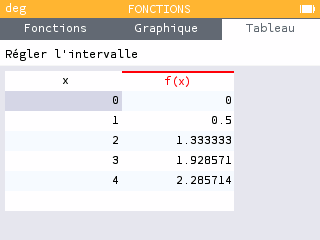
\includegraphics[width=6cm]{evaluation_11_sujet_B_numworks.png}    
    \end{center}
    Dans le repère suivant, tracer la courbe représentative de $f$, sachant que $f$ est une fonction impaire.
\end{enumerate}


\begin{center}
  \newrgbcolor{qqwuqq}{0. 0.39215686274509803 0.}
  \psset{xunit=0.7cm,yunit=0.7cm,algebraic=true,dimen=middle,dotstyle=o,dotsize=5pt 0,linewidth=1.pt,arrowsize=3pt 2,arrowinset=0.25}
  \begin{pspicture*}(-6.,-4.)(6.,4.)
    \multips(0,-4)(0,1.0){9}{\psline[linestyle=dashed,linecap=1,dash=1.5pt 1.5pt,linewidth=0.4pt,linecolor=lightgray]{c-c}(-6.,0)(6.,0)}
    \multips(-6,0)(1.0,0){13}{\psline[linestyle=dashed,linecap=1,dash=1.5pt 1.5pt,linewidth=0.4pt,linecolor=lightgray]{c-c}(0,-4.)(0,4.)}
    \psaxes[labelFontSize=\scriptstyle,xAxis=true,yAxis=true,Dx=1.,Dy=1.,ticksize=-2pt 0]{->}(0,0)(-6.,-4.)(6.,4.)
    %\psplot[linewidth=2.pt,linecolor=qqwuqq,plotpoints=200]{-6.0}{6.0}{3.0*x/(x^(2.0)+1.0)}
  \end{pspicture*}
\end{center}
\begin{enumerate}[resume]
  \item Le point $A(1,5; 1,4)$ appartient-il à la courbe de $f$ ?\rep{4}
\end{enumerate}

\end{document}
